\documentclass[parskip=full]{scrartcl}
\usepackage[top=2.5cm, bottom=2.5cm, left=2.5cm, right=2.5cm]{geometry}
\usepackage[utf8]{inputenc}
\usepackage[T1]{fontenc}
\usepackage[german]{babel}
\usepackage[pangram]{blindtext}
\usepackage{hyperref}
\usepackage[toc, nonumberlist, numberedsection]{glossaries}
\usepackage{graphicx}
\usepackage{enumitem}

\hypersetup{
  colorlinks=false,
  linktoc=all,
  hidelinks,
}

%!TEX root = Pflichtenheft.tex

\newglossaryentry{Dockerimage}
{
  name=Dockerimage,
  plural=Dockerimages,
  description={Ein Container mit Programmen, der unabhängig vom zugrunde liegenden Betriebssystem gleichbleibende Bedingungen herstellt}
}

\newglossaryentry{Fertigungssimulation}
{
  name=Fertigungssimulation,
  plural=Fertigungssimulationen,
  description={Darstellung der Industrieanlage und Simulieren des Verhaltens}
}


\newglossaryentry{GUI}
{
  name=GUI,
  plural=GUIs,
  description={Die grafische Benutzerumgebung des Programms, welche vom Bediener gesehen wird}
}

\newglossaryentry{Industrial Data Space}
{
  name=Industrial Data Space,
  plural=Industrial Data Spaces,
  description={Eine Infrastruktur zum Austausch von Daten in der Industrie}
}

\newglossaryentry{Jitter}
{
  name=Jitter,
  description={Simulation von variierenden Werten, um näher an echten Anlagen zu liegen}
}

\newglossaryentry{Makro}
{
  name=Makro,
  plural=Makros,
  description={Eine aufgezeichnete Folge von Einstellungen, die gesetzt werden. Wird benutzt, um einen komplexeren Ablauf in der Anlage zu simulieren}
}

\newglossaryentry{OPC UA}
{
  name=OPC UA,
  plural=OPC UA,
  description={Ein Protokoll zur Übertragung von Daten und Steuersignalen von Industrieanlagen}
}

\newglossaryentry{Produktionsanlage}
{
  name=Produktionsanlage,
  plural=Produktionsanlagen,
  description={Großmaschinen, wie sie in der Industrie eingesetzt werden. Hier symbolisiert durch Tanks mit Flüssigkeiten}
}

\newglossaryentry{Sensordatum}
{
  name=Sensordatum,
  plural=Sensordaten,
  description={Ausgabewert eines simulierten Sensors wie Temperatur oder Durchflussmenge}
}

\newglossaryentry{Systemadapter}
{
  name=Systemadapter,
  plural=Systemadapter,
  description={Konvertiert die Daten eines Gesamtsystems (hier Industrieanlage) in ein anderes Format}
}

\newglossaryentry{TCP/IP Verbindung}
{
  name=TCP/IP Verbindung,
  plural=TCP/IP Verbindungen,
  description={Ein Protokoll zum Datenaustausch über das Internet}
}

\newglossaryentry{Uberwachungskonsole}
{
  name=Überwachungskonsole,
  plural=Überwachungskonsolen,
  description={Anzeige der Sensorwerte der Fertigungssimulation}
}

\newglossaryentry{Wrapper}
{
  name=Wrapper,
  plural=Wrapper,
  description={Programm, das ein anderes Programm umgibt und auf Ereignisse im umgebenen Programm reagieren kann}
}
\makeglossaries

\title{Pflichtenheft}
\subtitle{Implementierung eines \gls{OPC UA} \glslink{Systemadapter}{Systemadapters} für den \gls{Industrial Data Space}}
\author{
    M. Armbruster\\
    D. Kahles\\
    H. Lehmann\\
    M. Schwarzmann\\
    N. Wilhelm
}

\begin{document}
\maketitle
\pagebreak
\tableofcontents
\pagebreak

\section{Einleitung}
In der heutigen Zeit dringt die Vernetzung in immer neue Bereiche vor. So auch in die Industrie und ihre Fertigungsprozesse.
Dabei soll das Projekt \gls{Industrial Data Space} helfen, einen Datenraum zu erzeugen, der Datensicherheit, Datensouveränität und
Transparenz bietet. Auf diese Weise soll dazu beigetragen werden, Industrie 4.0 voranzutreiben und somit durch Vernetzung von
Maschinen, Computern und Menschen die Leistungsfähigkeit der Industrie zu erhöhen und auf die Zukunft auszurichten.
Dabei hilft das auf \gls{TCP/IP} basierende Kommunikationsprotokoll \gls{OPC UA}, Maschinen miteinander kommunizieren zu lassen.

Die hier vorgestellte Simulation ermöglicht es, die Vorteile der Vernetzung von Maschinen mit \gls{OPC UA} interaktiv zu demonstrieren, um Industriekunden von den neuen Möglichkeiten zu überzeugen.
Die Hauptkomponenten sind eine \gls{Fertigungssimulation} (Server) und eine \gls{Uberwachungskonsole} (Client),
die jeweils eine graphische Benutzeroberfläche (\gls{GUI}) enthalten und auf getrennten Computern laufen können.
Sie kommunizieren lediglich über \gls{OPC UA}.
In der GUI der \gls{Fertigungssimulation} wird eine \gls{Produktionsanlage} dargestellt.
Drei Tanks werden mit je einer farbigen Flüssigkeit gefüllt und leiten diese in einen weiteren Tank,
in dem die Flüssigkeiten durch einen Motor gemischt werden. Daten und Werte der \gls{Produktionsanlage} werden ebenfalls angezeigt. Dazu gibt es
die Möglichkeit, die Parameter der \gls{Produktionsanlage} zu konfigurieren. Dies geschieht beispielsweise indem man Zu- und Abflussmengen einstellt. Die visuelle Darstellung passt sich an die Konfiguration an.
Die \gls{Uberwachungskonsole} liest die Daten der \gls{Fertigungssimulation}, stellt sie optisch ansprechend in einem Monitoring dar
und kann Alarme anzeigen, die vom \gls{OPC UA} Server empfangen werden. Das Monitoring ist ebenfalls konfigurierbar. Es ist etwa möglich, Filter auf Variablen anzuwenden. Allerdings hat die \gls{Uberwachungskonsole} keinen Einfluss auf die \gls{Fertigungssimulation}.

\pagebreak
\section{Zielbestimmung}
Der \gls{Systemadapter} dient dem Ziel, die Funktion von \gls{OPC UA} zu demonstrieren, ohne eine konkrete \gls{Produktionsanlage}
benutzen zu müssen. Somit kann beim Kunden das Protokoll flexibler vorgestellt werden. Hierzu soll das Programm
sowohl eine \gls{Produktionsanlage} simulieren und deren Status graphisch darstellen, als auch auch eine \gls{Uberwachungskonsole}
bereitstellen, die über \gls{OPC UA} Werte der \gls{Produktionsanlage} abfragt.\\
\begin{center}
    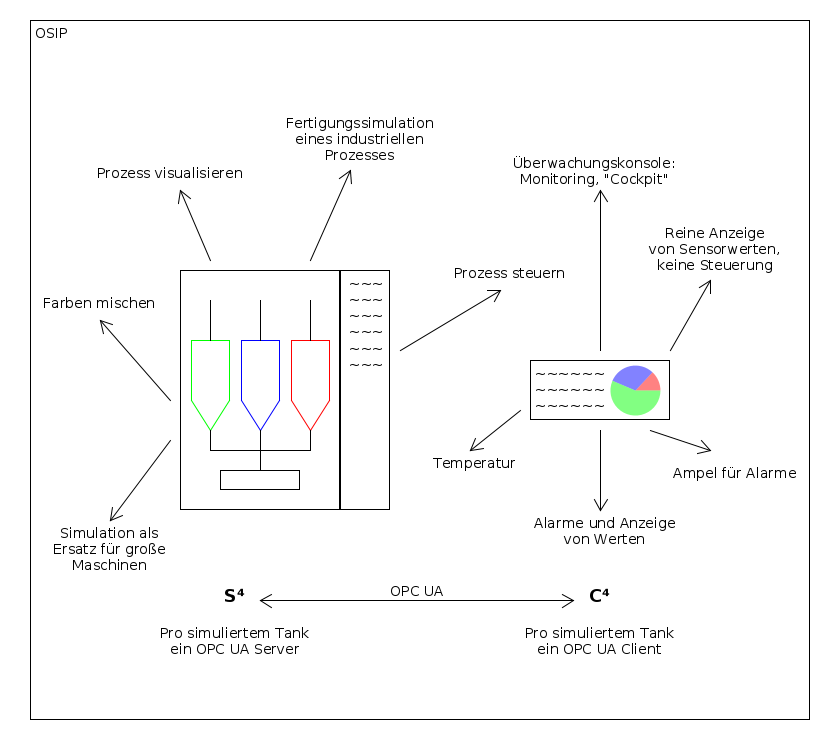
\includegraphics[scale=0.5]{../system-sketch.png}
\end{center}

\subsection{Musskriterien}
\subsubsection{Allgemein}
\begin{itemize}
  \item Die gesamte Kommunikation zwischen \gls{Uberwachungskonsole} und \gls{Fertigungssimulation} findet \"uber das \gls{OPC UA} Protokoll statt.
  \item \gls{Fertigungssimulation} und \gls{Uberwachungskonsole} laufen auf getrennten Rechnern.
\end{itemize}

\subsubsection{Überwachungskonsole}
\begin{itemize}
  \item Die \gls{Uberwachungskonsole} ruft alle \glspl{Sensordatum} der \gls{Fertigungssimulation} in einem festen Zeitintervall über einen \gls{OPC UA} Client ab.
  \item Der \gls{OPC UA} Client ist mit \gls{OPC UA} Servern verbunden. Dazu ist die Einstellung der Verbindungsinformationen möglich.
  \item Die abgerufenen Werte und deren zeitlicher Verlauf werden graphisch dargestellt. Die Werte sind Zu- und Abflussmengen, Temperaturen, Flüssigkeitsfarben sowie die Drehzahl eines Mischermotors.
  \item Die \gls{Uberwachungskonsole} enthält Alarme, die beim Überschreiten von Schwellenwerten in der \gls{Fertigungssimulation} durch den \gls{OPC UA} Server gesendet
    und dem Nutzer graphisch mitgeteilt werden.
\end{itemize}

\subsubsection{Fertigungssimulation}
\begin{itemize}
  \item In der \gls{Fertigungssimulation} kann der Benutzer die simulierte Fertigung steuern.
\end{itemize}


\subsection{Kannkriterien}
\subsubsection{Überwachungskonsole}
\begin{itemize}
  \item Das Zeitintervall für den Empfang der \glspl{Sensordatum} kann eingestellt werden.
  \item Die Alarme k\"onnen ein- und ausgeschaltet werden.
  \item Die Schwellen zur Ausl\"osung der Alarme k\"onnen vom Benutzer ge\"andert werden.
  \item Die \gls{Uberwachungskonsole} verfügt über eine Logging-Funktion.
  \item Die eingestellten Alarme k\"onnen gespeichert und beim n\"achsten Programmstart automatisch
    \"ubernommen werden.
\end{itemize}

\subsubsection{Fertigungssimulation}
\begin{itemize}
  \item Es gibt vordefinierte \glspl{Simulations-Szenario}, die über das Menü gestartet werden können.
  \item \gls{Jitter} in den Zuflussmengen der Tanks sorgt f\"ur Variation in den gemessenen Werten.
\end{itemize}


\subsection{Abgrenzungskriterien}
\subsubsection{Allgemein}
\begin{itemize}
  \item \gls{Fertigungssimulation} und \gls{Uberwachungskonsole} dienen der Demonstration des \glslink{OPC UA}{OPC UA Protokolls}. Dazu wird die Open Source
    Implementierung \gls{Milo} des \glslink{OPC UA}{OPC UA Protokolls} verwendet. \gls{OPC UA} wird nicht selbst implementiert.
\end{itemize}

\subsubsection{Überwachungskonsole}
\begin{itemize}
  \item Die \gls{Uberwachungskonsole} zeigt alle Sensorwerte und deren zeitlichen Verlauf an, stellt allerdings den Prozess nicht dar.
  \item Die \gls{Uberwachungskonsole} hat keinen Einfluss auf den Prozessablauf.
  \item Die \gls{Uberwachungskonsole} ist auf die \gls{Fertigungssimulation} abgestimmt. Es sollen damit nicht beliebige
    Fertigungsprozesse \"uberwacht werden k\"onnen.
  \item Die \gls{Uberwachungskonsole} dient ausschlie{\ss}lich der \"Uberwachung der Daten, die von der \gls{Fertigungssimulation}
    stammen. Sie kann nicht steuernd in die \gls{Fertigungssimulation} eingreifen.
\end{itemize}

\subsubsection{Fertigungssimulation}
\begin{itemize}
  \item Die \gls{Fertigungssimulation} stellt eine einzelne \gls{Produktionsanlage} schematisch dar. Die Darstellung verschiedener \glspl{Produktionsanlage}
    ist nicht das Ziel. Eine realistisch-detaillierte Simulation ist nicht das Ziel.
\end{itemize}



\newpage
\section{Produkteinsatz}
\subsection{Anwendungsbereiche}
Das Produkt wird verwendet, um \gls{OPC UA} und dessen Möglichkeiten zu präsentieren.
Insbesondere soll es einfacher aufzubauen und zu zeigen sein als reale \glspl{Fertigungssimulation}.
Dies kann zum Beispiel auf Messen oder direkt bei potenziellen Kunden geschehen.
\subsection{Zielgruppen}
Die Zielgruppe umfasst Personen, die sich mit \gls{OPC UA} auskennen und es potenziellen Anwendern vorführen möchten.
Dazu zählen insbesondere Mitglieder der OPC Foundation, die die Verbreitung des Protokolls fördern wollen,
aber auch Softwareentwickler die \gls{OPC UA} konforme Software herstellen und möglichen Kunden auf einfache Art und
Weise die Funktionalität von \gls{OPC UA} präsentieren wollen.
Die potenziellen Anwender haben meist keine Erfahrung mit \gls{OPC UA}, sind aber für \glspl{Produktionsanlage} verantwortlich
die von \gls{OPC UA} profitieren würden.

\subsection{Betriebsbedingungen}
Das Produkt kann entweder auf Messen, in Büros oder in Fertigungshallen direkt bei Kunden verwendet werden,
so lange die eingesetzte Hardware (siehe \ref{Hardware}) keine Probleme mit den Umgebungsbedingungen hat.

\pagebreak
\section{Produktumgebung}
\subsection{Software}
Das Produkt erfordert einen Computer, auf dem das Betriebssystem Microsoft Windows 7, 8.1 oder 10 installiert ist,
oder auf dem Canonical Ubuntu 14.04 oder 16.04 installiert ist. Außerdem ist das Oracle Java Runtime Environment in Version 1.8
notwendig. Wenn die \gls{Fertigungssimulation} und die \gls{Uberwachungskonsole} auf unterschiedlichen Computern laufen,
ist eine \gls{TCP/IP} Verbindung mit einer Bandbreite von 100 MBit/s und einer Latenz von maximal 100 ms zwischen den Computern notwendig.
Außerdem wird eventuell (siehe \ref{fertigung-optional} und \ref{konsole-optional}) unter Ubuntu 16.04 die Containersoftware Docker
ab Version 1.10.3 unterstützt, mit dem die beiden Softwareteile isoliert in Containern verteilt und ausgeführt werden können.

\subsection{Hardware}
\label{Hardware}
Es ist ein Laptop oder Desktopcomputer notwendig, der eines der oben genannten Betriebssysteme unterstützt.
Zudem sind mindestens 2GB Arbeitsspeicher notwendig. Die CPU muss die x86 Architektur unterstützen, zwei Kerne haben und mit
mindestens 2GHz getaktet sein.

\pagebreak
\section{Funktionale Anforderungen}
\subsection{Fertigungssimulation}
\subsubsection{Funktionalität}
\begin{enumerate}
\item[FA10] Die Zu- und Abflussmengen der oberen (siehe FA110) Flüssigkeitstanks können seperat eingestellt werden.
\item[FA20] Die Abflussmenge des unteren (siehe FA110) Flüssigkeitstanks kann eingestellt werden. Die Zuflussmenge ergibt sich aus der Summe der Abflussmengen der oberen Tanks.
\item[FA30] Der untere Tank enthält einen motorbetriebenen Mischer, dessen Drehzahl eingestellt werden kann.
\item[FA40] Jedem der oberen Tanks ist eine feste Flüssigkeitsfarbe zugeordnet. Die Farbe des unteren Tanks ergibt sich aus dem Mischungsverhältnis der oberen Tanks. Dabei wird
  angenommen, dass die Flüssigkeiten der oberen Tanks die selbe Deckkraft haben.
\item[FA40] Der linke obere Tank wird mit roter, der mittlere mit grüner und der rechte mit blauer Flüssigkeit gefüllt.
\item[FA45] Die Zuflusstemperaturen der oberen Tanks können seperat eingestellt werden (Kann-Kriterium).
\item[FA50] Es gibt eine .jar Datei, die bei Ausführung die \gls{Fertigungssimulation} startet.
\item[FA60] Nach Anforderung durch die \gls{Uberwachungskonsole} wird in bestimmten, in der Anfrage definierten, Zust\"anden ein Alarm an die \gls{Uberwachungskonsole} gesendet.
\item[FA70] Kommt es in der \gls{Fertigungssimulation} zu einem \"Uberlauf so h\"alt die \gls{Fertigungssimulation} an und es wird der Text "`\"Uberlauf"' angezeigt.
\item[FA80] Das System kann aus einem "`\"Uberlauf"' durch den Knopf "`zur\"ucksetzen"' im gezeigten Dialog wieder in den Startzustand versetzt werden. Anschlie{\ss}end wird die Ausführung fortgesetzt.
\item[FA90] Eine \gls{Uberwachungskonsole} kann sich bei der \gls{Fertigungssimulation} registrieren, um von dieser Daten zu erhalten.
\item[FA110] Die Füllstände der Tanks werden gemessen.
\item[FA120] Die \gls{Fertigungssimulation} kommuniziert über \gls{OPC UA} in einem \gls{TCP/IP} Netzwerk mit \glspl{Uberwachungskonsole}.
\item[FA130] Die Ports, über welche die einzelnen \gls{OPC UA Server} der \gls{Fertigungssimulation} kommunizieren, können eingestellt werden.
\item[FA140] Die \gls{Fertigungssimulation} besitzt vordefinierte \glspl{Simulations-Szenario}, die über das Menü gestartet werden können (Kann-Kriterium).
\item[FA150] Ein \gls{Simulations-Szenario} ist ein fester, zeitlicher Ablauf, der komplexere Szenarien in der \gls{Fertigungssimulation} darstellt. Somit kann ohne aktive Nutzerinteraktion eine sich
  im aktiven Betrieb befindliche \gls{Produktionsanlage} simuliert werden.
\end{enumerate}

\subsubsection{GUI Darstellung}
\begin{enumerate}
\item[FA110] Die \gls{GUI} der \gls{Fertigungssimulation} zeigt drei Tanks, die auf einer Höhe sind, und einen Tank unter den oberen drei.
Es führen Leitungen von den drei oberen Tanks zum unteren Tank.
\item[FA150] An jeder Leitung befinden sich ein Ventil sowie ein Durchflussmesser in Form eines sich drehenden Elements. Der Öffnungsgrad des Ventils wird prozentual auf dem Ventil angezeigt.
\item[FA120] Der Mischer im unteren Flüssigkeitstank wird durch ein sich drehendes GUI Element dargestellt.
Die Umdrehungsgeschwindigkeit repräsentiert die Drehzahl des Mischermotors.
\item[FA150] An jedem Tank ist ein Temperatursensor angebracht (sofern implementiert).
\item[FA130] Der Füllstand der Flüssigkeitstanks wird durch das Füllen der Tanks in der Farbe ihrer Flüssigkeit dargestellt.
\item[FA140] Die einstellbaren Parameter können in einem Unterfenster eingestellt werden. Darin existiert für jeden Tank ein eigener Reiter, der die 
tankspezifischen Einstellungen wie zum Beispiel Zu- und Abflussmengen, Zuflusstemperaturen oder Motordrehzahlen (siehe FA10 bis FA30) enthält.
Diese Parameter werden durch Schieberegler eingestellt.
\item[FA150] Jeder der dargestellten Tanks ist mit einer hellgrauen Box hinterlegt, welche den Zuständigkeitsbereich des jeweiligen \glslink{OPC UA Server}{OPC UA Servers} repräsentiert.
\item[FA160] Die \gls{Fertigungssimulation} besitzt einen "`Über"'-Dialog, welcher Lizenzinfos zu verwendeten Bibliotheken,
  sowie eine kurze Information zu den Erstellern des Programms, enthält.
\item[FA170] Die \gls{Fertigungssimulation} besitzt einen Einstellungsdialog, der im Menü über "`Datei $\rightarrow$ Einstellungen"' angezeigt werden kann.
\item[FA180] Der Einstellungsdialog besitzt Buttons zum Verwerfen ("`Abbrechen"') und Anwenden der Änderungen. Das Anwenden geschieht über einen "`OK"'-Button, welcher zudem den Dialog schließt.
\item[FA200] Der Einstellungsdialog besitzt einen Regler, welcher den \gls{Jitter} durch einen Schieberegler konfigurierbar macht.
  Hierbei entspricht ein \gls{Jitter} von 0 der Deaktivierung der Funktion.
\item[FA210] Der Menüeintrag "`Szenarien"' zeigt eine Liste der \glspl{Simulations-Szenario}, die durch einen Klick gestartet werden können.
\end{enumerate}

\subsubsection{Optionale Funktionalität}
\label{fertigung-optional}
\begin{enumerate}
\item[FA240] Es gibt ein \gls{Dockerimage} zur einfachen Verteilung und isolierten Ausführung der \gls{Fertigungssimulation}.
\end{enumerate}

\subsection{Überwachungskonsole}
\subsubsection{Funktionalität}
\begin{enumerate}
\item[FA310] Es gibt eine .jar-Datei, die bei Ausführung die \gls{Uberwachungskonsole} startet.
\item[FA320] Die \gls{Uberwachungskonsole} ist ein \gls{OPC UA Client}.
\item[FA330] Der \gls{OPC UA Client} erhält die \gls{IP-Adresse}, die durch die \gls{Uberwachungskonsole} nicht geändert werden kann, des verwendeten Computers.
\item[FA340] Der \gls{OPC UA Client} verbindet sich mit den \glslink{OPC UA Server}{OPC UA Servern} einer \gls{Fertigungssimulation} und kommuniziert mit diesen über \gls{TCP/IP}.
\item[FA350] Beim Start versucht die \gls{Uberwachungskonsole}, eine Verbindung mit den \glslink{OPC UA Server}{OPC UA Servern} herzustellen und sich dort zu registrieren.
\item[FA360] Schlägt die Verbindung von [FA350] oder [FA600] fehl, wird der Benutzer über einen Dialog informiert.
\item[FA370] Alle angezeigten \glspl{Sensordatum} werden mit einer eingestellten, festen Frequenz aktualisiert.
\item[FA380] Alarme mit ihrem jeweiligen Auslöser können bei der \gls{Fertigungssimulation} registriert werden.
\item[FA390] Alarme werden asynchron zu den \glspl{Sensordatum} empfangen und direkt angezeigt, sobald sie ausgelöst werden.
\end{enumerate}

\subsubsection{GUI Darstellung}
\begin{enumerate}
\item[FA400] Die \gls{Uberwachungskonsole} stellt die \glspl{Sensordatum} und Alarme jedes Flüssigkeitsanks in einem eigenen Bereich dar.
\item[FA410] Die \gls{Uberwachungskonsole} zeigt die Farbe der Tanks an.
\item[FA420] Die \gls{Uberwachungskonsole} zeigt die Zuflussmenge der oberen Tanks auf jeweils einer Skala an.
\item[FA430] Die \gls{Uberwachungskonsole} zeigt die Abflussmenge aller Tanks auf jeweils einer Skala an.
\item[FA440] Die \gls{Uberwachungskonsole} zeigt den Füllstand aller Tanks auf jeweils einer Skala an.
\item[FA450] Die \gls{Uberwachungskonsole} zeigt die Temperatur aller Tanks auf jeweils einer Skala an (sofern implementiert).
\item[FA460] Die \gls{Uberwachungskonsole} zeigt die Drehzahl des Mischermotors im unteren Tank auf einer Skala an.
\item[FA470] Der zeitliche Verlauf des Füllstandes wird jeweils für alle Tanks angezeigt.
\item[FA480] Der zeitliche Verlauf der Temperatur wird jeweils für alle Tanks angezeigt.
\item[FA490] Die \gls{Uberwachungskonsole} registriert für jeden Tank jeweils einen Alarm für einen Überlauf.
\item[FA500] Die \gls{Uberwachungskonsole} registriert für jeden Tank jeweils einen Alarm für einen Unterlauf.
\item[FA510] Ein Alarm wird durch einen Bezeichner und einen Kreis als Zustandssymbol dargestellt.
\item[FA520] Ist der Kreis rot, wurde der Alarm ausgelöst.
\item[FA530] Ist der Kreis grün, ist der Alarm nicht ausgelöst.
\item[FA540] Ein Alarm wird als ausgelöst angezeigt, nachdem die \gls{Uberwachungskonsole} durch die \gls{Fertigungssimulation} darüber benachrichtigt wurde und bis der Alarm in der
  \gls{Fertigungssimulation} nicht mehr aktiv ist und die \gls{Uberwachungskonsole} darüber informiert wurde.
\item[FA550] Es gibt eine zweistufige Ampel für den allgemeinen Zustand der \gls{Uberwachungskonsole}.
\item[FA560] Ist die Ampel rot, wurde mindestens ein Alarm ausgelöst.
\item[FA570] Ist die Ampel grün, wurde kein Alarm ausgelöst.
\item[FA580] Die \gls{Uberwachungskonsole} bietet eine Menüleiste mit den Punkten "`Datei"', das den Untermenüpunkt "`Einstellungen"' beinhaltet, und "`?"', das den Untermenüpunkt "`Über"' beinhaltet.
\item[FA590] "`? $\rightarrow$ Über"' öffnet ein neues Fenster, in dem der Programmname, die Version, das Programmsymbol und die Lizenz angezeigt werden.
\item[FA600] "`Datei $\rightarrow$ Einstellungen"' öffnet ein separates Fenster, in dem alle Einstellungen in einem Reiter "`Allgemeine Einstellungen"' vorgenommen werden können.
\item[FA610] In den Einstellungen werden die IP-Adresse des \glslink{OPC UA Client}{OPC UA Clients} und der \gls{OPC UA Server} sowie deren Ports angezeigt.
\end{enumerate}

\subsubsection{Benutzerinteraktion}
\begin{enumerate}
\item[FA570] Der Benutzer kann in den Einstellungen den Port für den \gls{OPC UA Client} bzw. die Ports und die IP-Adresse für die \glspl{OPC UA Server} einstellen.
\item[FA580] Nach Drücken eines Speichern-Knopfes im Einstellungsfenster werden alle vorhandenen Einstellungen mit denen aus dem Fenster überschrieben.
\item[FA590] Nach Drücken eines Abbruch-Knopfes im Einstellungsfenster bleiben die Einstellungen unverändert.
\item[FA600] Werden Einstellungen für die \glspl{OPC UA Server} oder den \gls{OPC UA Client} überschrieben, wird der \gls{OPC UA Client} mit den neuen Einstellungen neu gestartet.
\item[FA610] Die Eingaben in den Einstellungen werden direkt nach Eingabe auf richtige Formatierung und Einhaltung des Wertebereichs gepr\"uft.
\item[FA620] Der Benutzer wird über eine Fehleingabe und deren Ursache informiert.
\end{enumerate}

\subsubsection{Optionale Funktionalität}
\label{konsole-optional}
\begin{enumerate}
\item[FA630] Es gibt ein \gls{Dockerimage} zur einfachen Verteilung und isolierten Ausführung der \gls{Uberwachungskonsole}.
\item[FA640] Bereits registrierte Alarme können wieder gelöscht werden.
\item[FA650] Das Einstellungsfenster wird um zwei Reiter, "`Verläufe"' und "`Alarme"' erweitert.
\item[FA660] In den "`Allgemeinen Einstellungen"' ist es dem Nutzer möglich, das Zeitintervall für die Aktualisierung der Werte über einen Schieberegler oder eine Textbox einzustellen.
\item[FA670] Unter "`Verläufe"' ist es möglich, jede Aufnahme des zeitlichen Verlaufs eines Wertes ein und aus zu schalten.
\item[FA680] In "`Alarme"' kann der Nutzer die verfügbaren Alarme ein- und ausschalten und deren Schwellenwerte festlegen.
\item[FA690] Es gibt eine Loggingkonsole in Form einer mehrzeiligen Textausgabe.
\item[FA700] Geloggt werden Fehler, Ausnahmen und Aktivitäten der \gls{Uberwachungskonsole} sowie alle eintreffenden Alarme.
\end{enumerate}

\pagebreak
\section{Nichtfunktionale Anforderungen}
\subsection{Fertigungssimulation}
\begin{enumerate}
 \item[NF10] Die Drehzahl des Mischermotors kann in einem Bereich zwischen 0 und 300 Umdrehungen pro Minute gewählt werden.
 \item[NF20] Wenn Parameter verändert werden, sind sie nach spätestens einer halben Sekunde per \gls{OPC UA} abrufbar.
 \item[NF30] Wenn der Zufluss eines Tanks komplett geschlossen, und der Ablauf komplett geöffnet wird, ist der Tank in etwa 10 Sekunden leergelaufen.
 \item[NF40] Wenn der Zufluss eines Tanks komplett geöffnet, und der Ablauf komplett geschlossen wird, ist der Tank in etwa 10 Sekunden übergelaufen.
\end{enumerate}

\subsection{Überwachungskonsole}
\begin{enumerate}
 \item[NF110] IP-Adressen muss eine gültige IPv4 oder IPv6 Addresse oder gültige Hostnamen sein. % Abkürzungsverzeichnis für Dinge wie IPv4?
 \item[NF120] Ports dürfen Werte im Bereich 1024 bis 61000 annehmen.
 \item[NF130] Die Schwellenwerte für die Alarme dürfen zwischen 0 und 100 \% gewählt werden.
 \item[NF140] Die Aktualisierungsfrequenz kann im Bereich zwischen 20 und 4000 Millisekunden gewählt werden.
 \item[NF150] Wenn sich Werte in der \gls{Fertigungssimulation} ändern, werden die Änderungen spätestens nach der Zeitspanne von
   einer halben Sekunde plus dem Aktualisierungsintervall in der \gls{Uberwachungskonsole} angezeigt.
\end{enumerate}

\pagebreak
\section{Produktdaten}
\begin{enumerate}
 \item[D10] Die \gls{Uberwachungskonsole} speichert den zuletzt eingestellten Port des \glslink{OPC UA Client}{OPC UA Clients}.
 \item[D20] Die \gls{Uberwachungskonsole} speichert die zuletzt eingestellte IP-Adresse und Ports der \gls{OPC UA Server}.
 \item[D30] Die \gls{Uberwachungskonsole} speichert die zuletzt eingestellte Aktualisierungsfrequenz für die \glspl{Sensordatum}.
 \item[D40] Die \gls{Uberwachungskonsole} speichert die zuletzt eingeschaltenen Alarme und alle Schwellenwerte.
 \item[D50] Die \gls{Uberwachungskonsole} speichert, welche Verläufe zuletzt angezeigt wurden.
 \item[D110] Die \gls{Fertigungssimulation} speichert die zuletzt genutzten Ports der \glspl{OPC UA Server}.
 \item[D120] Die \gls{Fertigungssimulation} speichert den zuletzt eingestellten \gls{Jitter}.
 \item[D130] Die \gls{Fertigungssimulation} speichert \glspl{Simulations-Szenario} in einzelnen Dateien (sofern implementiert).
\end{enumerate}

\pagebreak
\section{Globale Testfälle}
\Blindtext[1]

\pagebreak
\section{Systemmodelle}
\subsection{Szenarien}
\subsubsection*{Akteure}
\textbf{Manuel}: Der Benutzer des Programms, der \gls{OPC UA} vermarkten will.\\
\textbf{Philipp}: Ein potenzieller Anwender von \gls{OPC UA}, der das Protokoll noch nicht kennt.

\subsubsection{Szenario 1: Unabhängige Installation}
Manuel möchte Philipp, einem Kunden aus der Industrie, zeigen, was mit modernen Industrie 4.0 Techniken möglich ist.
Da Philipp nur wenig Zeit hat, fährt Manuel mit dem Auto zu Philipp. Weil Manuel weder Platz 
noch Zeit für eine komplette Demonstrationsanlage hat, nimmt er einen Laptop mit Simulationssoftware mit.

Vor Ort angekommen, startet er auf dem Laptop zwei virtuelle Maschinen, auf denen je ein Programm installiert ist. 
Einmal eine \gls{Fertigungssimulation} und auf der anderen virtuellen Maschine eine \gls{Uberwachungskonsole}, um die Fertigung zu überwachen.
Nun weist Manuel den beiden virtuellen Maschinen je eine feste IP-Adresse zu.
Anschlie{\ss}end startet Manuel erst die \gls{Fertigungssimulation} und dann die \gls{Uberwachungskonsole}.
Beim Start der \gls{Uberwachungskonsole} wird er nach der IP-Adresse gefragt, unter der die \gls{Fertigungssimulation} zu finden ist. 
Er gibt die Adresse der anderen virtuellen Maschine an und auch die \gls{Uberwachungskonsole} startet erfolgreich. 
Nun ist klar, dass die beiden Programme tatsächlich über das Netzwerk kommunizieren.

In der \gls{Fertigungssimulation} wird nun eine \gls{Produktionsanlage} angezeigt, in der Flüssigkeiten aus drei Tanks
in einem weiteren Tank vermischt werden; Farben des Inhalts der Ursprungs- und des Zieltanks visualisieren den Vorgang. 
Im Zieltank dreht sich ein Motor, der für die Durchmischung sorgt.
Es gibt Sensoren für Temperatur, Farbe, Füllstand und Durchfluss der Tanks sowie für die Drehzahl des Motors.
In der \gls{Uberwachungskonsole} sieht man nun eine Reihe von Feldern mit sich aktualisierenden Daten,
die Zu- und Abfluss, Farbe und Temperatur der verschiedenen Tanks zeigen.

\subsubsection{Szenario 2: Konfigurierbarkeit}
Als Philipp zu ihm kommt, will Manuel ihm die Funktion von \gls{OPC UA} demonstrieren.
Als erstes ändert er in der \gls{Fertigungssimulation} den Zu- und Abfluss bei zwei der Tanks. Nun sehen die beiden, wie
sich die von der \gls{Uberwachungskonsole} angezeigten Werte für Zu- und Abfluss mit der nächsten Aktualisierung ändern. Die
Farbe im Zielcontainer ändert sich langsam, während sich das Mischungsverhältnis der Flüssigkeiten ändert. Auch diese
Werte werden in der \gls{Uberwachungskonsole} jeweils aktualisiert.

Als nächstes betrachten die beiden, wie sich in der \gls{Uberwachungskonsole} die Anzeigen für den Füllstand und die
Motorgeschwindigkeit des unteren Tankes ändern.
Außerdem verweist Manuel auf Reiter unterhalb der Überwachungsanzeigen der Tanks,
in denen Philipp die Füllstands- und Temperaturverläufe ansehen kann.

Philipp merkt nun an, dass ihm die Flexibilität der empfangenen Daten sehr gefällt. Das Aktualisierungsintervall von
einer Sekunde sei aber in manchen der Fertigungsprozesse zu lang, da in manchen kritischen Zuständen sehr schnell
automatisch reagiert werden muss, etwa wenn Schwellenwerte überschritten werden. Daraufhin ändert Manuel in den
Einstellungen das Aktualisierungsintervall von 1000ms auf 250ms. Anschließend sehen beide, wie sich die Werte in der
\gls{Uberwachungskonsole} tatsächlich vier Mal pro Sekunde aktualisieren.

\subsubsection{Szenario 3: Alarme}
Philipp ist zunehmend an \gls{OPC UA} interessiert, hat aber noch letzte Zweifel. Er merkt an, dass die Abfrage der Daten
zwar gut funktioniert, eine wirkliche \"Uberwachung aber noch einen \gls{Wrapper} f\"ur das Programm ben\"otigen w\"urde,
um ungew\"ohnliche Zust\"ande in der Fertigung automatisch zu bemerken und darauf aufmerksam zu machen.
Manuel merkt an, dass das ein guter Einwand ist und dass \gls{OPC UA} auch daf\"ur eine passende Funktionalit\"at besitzt.

Er \"offnet das Einstellungsmen\"u der \gls{Uberwachungskonsole} und ruft den Reiter "`Alarme"' auf. Um die Flexibilit\"at
von \gls{OPC UA} erneut zu demonstrieren, fragt er Philipp, welchen vorhandenen Zustand er gerne abfangen w\"urde. Philipp möchte gerne
wissen, wenn ein Tank \"uberzulaufen droht. Er schl\"agt daf\"ur als Grenze einen F\"ullstand von 95\% vor.
Manuel gibt also in der \gls{Uberwachungskonsole} 95\% als Grenze an und w\"ahlt einen Tank, f\"ur den der Alarm stattfinden soll.
Dann speichert er die neuen Einstellungen.

Anschlie{\ss}end dreht er in der \gls{Fertigungssimulation} den Zufluss des entsprechenden Tanks auf, woraufhin der F\"ullstand
zu steigen beginnt. In der \gls{Fertigungssimulation} ist der steigende F\"ullstand zu sehen, in der \gls{Uberwachungskonsole} werden
steigende Werte angezeigt.
Darauf wird der F\"ullstand von 95\% erreicht und in der \gls{Uberwachungskonsole} der Alarm ausgel\"ost. Manuel
beschlie{\ss}t, nicht zu handeln, und der Tank l\"auft \"uber. Danach w\"ahlt Philipp in den Einstellungen der
\gls{Fertigungssimulation} die Option "`zur\"ucksetzen"', woraufhin wieder die Standardkonfiguration angezeigt wird.

\subsection{Anwendungsfälle}
\subsubsection{Änderung der Zu-/Abflussgeschwindigkeit}
\begin{description}
  \item[Name] Erhöhen oder Verringern der Zu- oder Abflussgeschwindigkeit bei einem der Flüssigkeitstanks.
  \item[Akteure] Manuel (Bediener der Software)
  \item[Eingangsbedingung] Die \gls{Fertigungssimulation} und die \gls{Uberwachungskonsole} sind in Betrieb und miteinander verbunden.
  \item[Ereignisfluss]~\\
\begin{itemize}[noitemsep]
  \item Manuel öffnet in der \gls{Fertigungssimulation} den Menüeintrag "`Ansicht"'.
  \item Manuel klickt auf "`Steuerung anzeigen"'.
  \item Ein Fenster öffnet sich. Manuel wählt den Reiter des Tanks, den er verändern will.
  \item Manuel verschiebt den Schieberegler des Zufluss- oder Abflussventils auf den gewünschten Wert.
  \item Manuel klickt den "`OK"' Knopf.
\end{itemize}
  \item[Ausgangssituation] Die Zu- oder Abflussrate im gewählten Tank ist nun höher bzw. niedriger. Dies ist am schnelleren oder
    langsameren Füllen oder Leeren des Tanks in der Visualisierung der Tanks sichtbar.
    Außerdem zeigt die \gls{Uberwachungskonsole} höhere/niedrigere Durchflussraten an.
  \item [Nichtfunktionale Anforderungen] Der geänderte Zu- oder Abflusswert wird mit der nächsten Aktualisierung auf der \gls{Uberwachungskonsole} angezeigt.
\end{description}

%
% Diese Funktionalität ist im Moment nicht vorgesehen.
%
%\subsubsection{Änderung der angezeigten Sensorwerte}
%\begin{description}
% \item[Name] Hinzuwählen oder Abwählen von \glspl{Sensordatum}, die in der \gls{GUI} angezeigt werden.
% \item[Akteure] Manuel (Bediener der Software)
% \item[Eingangsbedingung] Die Fertigungssimulation und die Überwachungskonsole sind in Betrieb und miteinander verbunden.
% \item[Ereignisfluss]~\\
% \begin{itemize}[noitemsep]
%  \item Manuel öffnet in der Überwachungskonsole die Einstellungen.
%  \item Ein neues Fenster erscheint. Manuel navigiert in den Reiter "`Empfangene Daten"'.
%  \item Manuel klickt auf die Haken in der Liste, um Sensorwerte hinzuzufügen oder auszublenden.
%  \item Manuel klickt den "`OK"' Knopf.
% \end{itemize}
% \item[Ausgangssituation] Die \glspl{Sensordatum}, deren Haken entfernt wurden, werden sofort ausgeblendet. Die \glspl{Sensordatum}, deren Haken hinzugefügt wurden, erscheinen sofort in der \gls{GUI}.
% \item [Nichtfunktionale Anforderungen] Die geänderten Einstellungen werden binnen einer halben Sekunde in der \gls{GUI} dargestellt.
%\end{description}

\subsubsection{Änderung der Aktualisierungsfrequenz}
\begin{description}
 \item[Name] Erhöhen oder Verringern der Aktualisierungsfrequenz.
 \item[Akteure] Manuel (Bediener der Software)
 \item[Eingangsbedingung] Die \gls{Fertigungssimulation} und die \gls{Uberwachungskonsole} sind in Betrieb und miteinander verbunden.
 \item[Ereignisfluss]~\\
 \begin{itemize}[noitemsep]
  \item Manuel öffnet in der \gls{Uberwachungskonsole} die Einstellungen.
  \item Manuel navigiert in den Reiter "`Allgemeine Einstellungen"'.
  \item Manuel verschiebt den Schieberegler, der die Aktualisierungsfrequenz einstellt.
  \item Manuel klickt den "`Speichern"' Knopf.
 \end{itemize}
 \item[Ausgangssituation] Die \glspl{Sensordatum} in der \gls{Uberwachungskonsole} werden nun in Abständen der gewählten Aktualisierungsfrequenz aktualisiert.
 \item [Nichtfunktionale Anforderungen] Die Frequenz ändert sich spätestens mit der nächsten Aktualisierung.
\end{description}

\subsubsection{Erstes Starten der Simulation auf virtuellen Maschinen}
\begin{description}
 \item[Name] Einrichtung und Starten der Simulation auf virtuellen Maschinen
 \item[Akteure] Manuel (Bediener der Software)
 \item[Eingangsbedingung] Ein Computer (oder virtuelle Maschine), auf der die .jar Datei der \gls{Uberwachungskonsole} gespeichert ist und ein Computer (oder virtuelle Maschine), auf der die .jar
 Datei der \gls{Fertigungssimulation} gespeichert ist, sind in Betrieb und haben feste IP Adressen zugewiesen bekommen.
 \item[Ereignisfluss]~\\
 \begin{itemize}[noitemsep]
  \item Manuel startet die JAR der \gls{Fertigungssimulation}.
  \item Manuel startet die JAR der \gls{Uberwachungskonsole}.
  \item Manuel gibt die IP Adresse ein, unter der die \gls{Fertigungssimulation} zu finden ist.
 \end{itemize}
 \item[Ausgangssituation] Die \gls{Fertigungssimulation} und die \gls{Uberwachungskonsole} sind verbunden und laufen mit ihren Initialwerten.
 \item[Nichtfunktionale Anforderungen] Die \glspl{Sensordatum} der \gls{Uberwachungskonsole} werden nach spätestens einer halben Sekunde aktualisiert.
\end{description}
 
\subsubsection{Alarm einschalten}
\begin{description}
 \item[Name] Einschalten eines Alarms in der \gls{Uberwachungskonsole}.
 \item[Akteure] Manuel (Bediener der Software)
 \item[Eingangsbedingung] Die \gls{Fertigungssimulation} und die \gls{Uberwachungskonsole} sind in Betrieb und miteinander verbunden.
 \item[Ereignisfluss]~\\
 \begin{itemize}[noitemsep]
  \item Manuel \"offnet in der \gls{Uberwachungskonsole} die Einstellungen.
  \item Manuel navigiert in den Reiter "`Alarme"'.
  \item Manuel w\"ahlt den Alarm aus, der eingeschalten werden soll.
  \item Manuel aktiviert die Checkbox, die zum Alarm gehört.
  \item Manuel stellt zusätzlich einen Schwellenwert ein oder lässt den aktuell angezeigten.
  \item Manuel klickt den "`Speichern"' Knopf.
 \end{itemize}
 \item[Ausgangssituation] Wenn der Sensor die Alarmbedingung erf\"ullt, wird an die \gls{Uberwachungskonsole} ein Alarm gesendet.
 \item [Nichtfunktionale Anforderungen] Sp\"atestens nach 100ms ist die Aktualisierung \"ubernommen und wird
  an die \gls{Fertigungssimulation} gesendet.
\end{description}

\subsubsection{Alarm empfangen}
\begin{description}
 \item[Name] Empfangen eines Alarms in der \gls{Uberwachungskonsole}.
 \item[Akteure] \gls{Fertigungssimulation}
 \item[Eingangsbedingung] Die \gls{Fertigungssimulation} und die \gls{Uberwachungskonsole} sind in Betrieb und miteinander verbunden.
  Es ist mindestens ein Alarm eingerichtet.
 \item[Ereignisfluss]~\\
 \begin{itemize}[noitemsep]
  \item In der \gls{Fertigungssimulation} kommt es zu einem Alarmzustand.
  \item Die \gls{Fertigungssimulation} sendet den entsprechenden Alarm an die registrierte \gls{Uberwachungskonsole}.
  \item Die \gls{Uberwachungskonsole} empf\"angt den Alarm.
  \item Die \gls{Uberwachungskonsole} zeigt in der \gls{GUI} den Alarm an.
 \end{itemize}
 \item[Ausgangssituation] \gls{Fertigungssimulation} und \gls{Uberwachungskonsole} laufen normal weiter. In der \gls{GUI} der
  \gls{Uberwachungskonsole} ist der Alarmeintrag zu sehen.
 \item [Nichtfunktionale Anforderungen] Die \gls{GUI} der \gls{Uberwachungskonsole} muss einen empfangenen Alarm nach sp\"atestens
  100ms plus der Aktualisierungsfrequenz anzeigen.
\end{description}

\subsubsection{Alarm \"andern}
\begin{description}
 \item[Name] \"Andern eines bereits vorhandenen Alarms in der \gls{Uberwachungskonsole}.
 \item[Akteure] Manuel (Bediener der Software)
 \item[Eingangsbedingung] Die \gls{Uberwachungskonsole} ist in Betrieb. Es ist mindestens ein Alarm bereits eingeschalten.
 \item[Ereignisfluss]~\\
 \begin{itemize}[noitemsep]
  \item Manuel \"offnet in der \gls{Uberwachungskonsole} die Einstellungen.
  \item Manuel navigiert in den Reiter "`Alarme"'.
  \item Manuel w\"ahlt den gew\"unschten Alarm aus.
  \item Manuel tr\"agt den gew\"unschten Schwellenwert ein.
  \item Manuel klickt auf "`Speichern"'.
 \end{itemize}
 \item[Ausgangssituation] Die alte Alarmbedingung l\"ost keine Alarme mehr aus. Die neue Alarmbedingung l\"ost Alarme aus.
 \item [Nichtfunktionale Anforderungen] Die ge\"anderte Alarmbedingung ist nach sp\"atestens 500ms plus der Netzwerklatenz \"ubernommen und
  wird an die \gls{Fertigungssimulation} gesendet.
\end{description}

\subsubsection{Alarm ausschalten}
\begin{description}
 \item[Name] Ausschalten eines eingeschaltenen Alarms.
 \item[Akteure] Manuel (Bediener der Software)
 \item[Eingangsbedingung] Die \gls{Uberwachungskonsole} ist in Betrieb. Es ist mindestens ein Alarm bereits eingeschalten.
 \item[Ereignisfluss]~\\
 \begin{itemize}[noitemsep]
  \item Manuel \"offnet in der \gls{Uberwachungskonsole} die Einstellungen.
  \item Manuel navigiert in den Reiter "`Alarme"'.
  \item Manuel deaktiviert die Checkbox aller gew\"unschten Alarme.
  \item Manuel klickt auf "`Speichern"'.
 \end{itemize}
 \item[Ausgangssituation] Die alten Alarmbedingungen l\"osen keine Alarme mehr aus.
 \item [Nichtfunktionale Anforderungen] Das Ausschalten der Alarme wird nach sp\"atestens 100ms an die \gls{Fertigungssimulation} \"ubermittelt.
\end{description}

\subsubsection{Anwendungsfalldiagramm}
\begin{center}
  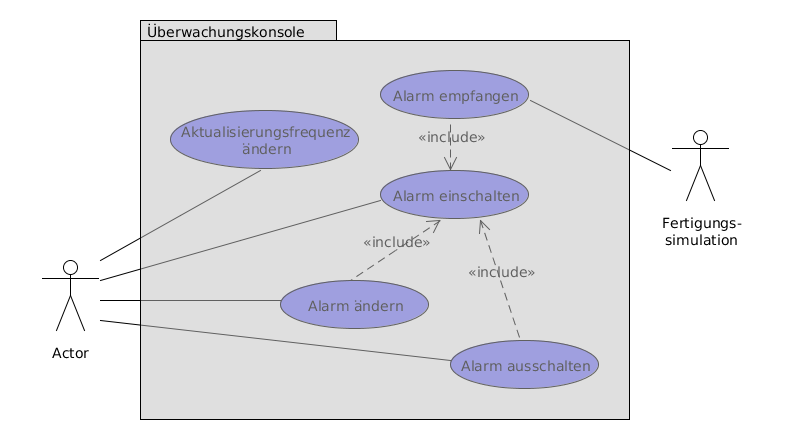
\includegraphics[scale=0.62]{media/UseCases/Ueberwachungskonsole.png}
\end{center}

\subsection{Dynamische Modelle}
\Blindtext[1]

\subsection{Statische Modelle}
\Blindtext[1]

\section{Nutzerinterface-Skizzen}
\subsection{Fertigungssimulation}
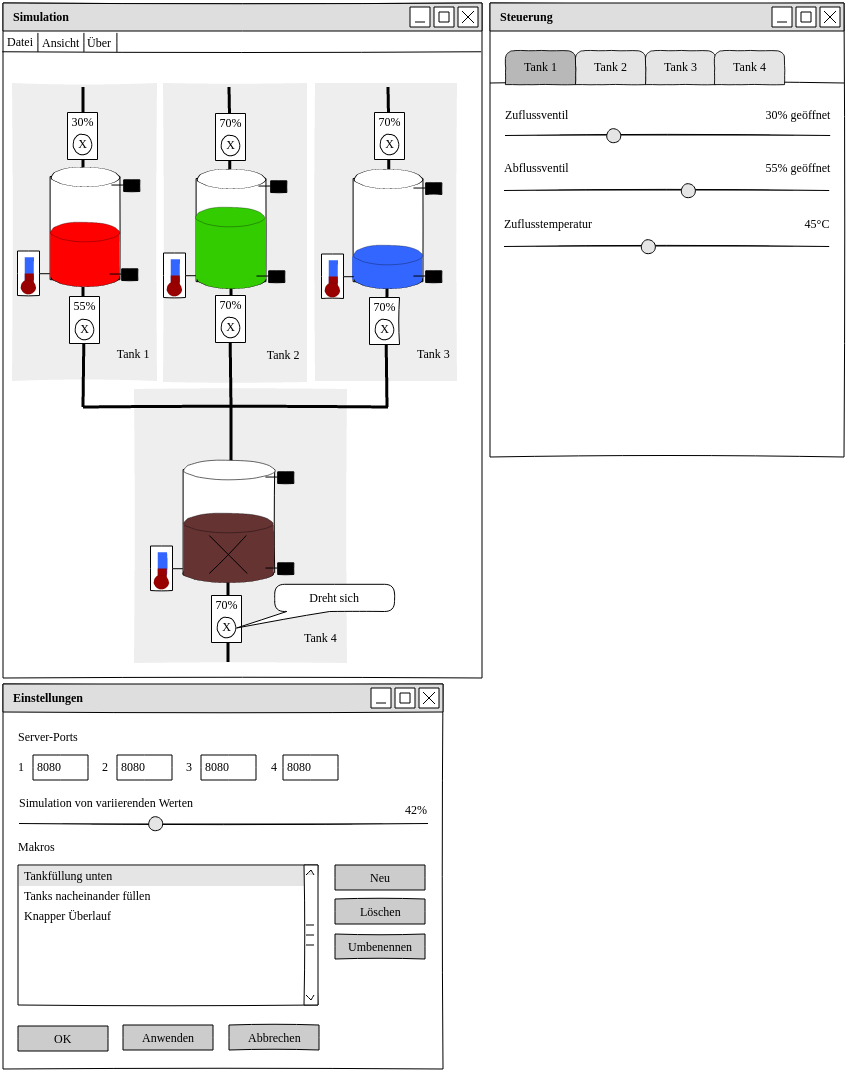
\includegraphics[scale=0.5]{media/ui-sketch-server.png}
\subsection{Überwachungskonsole}
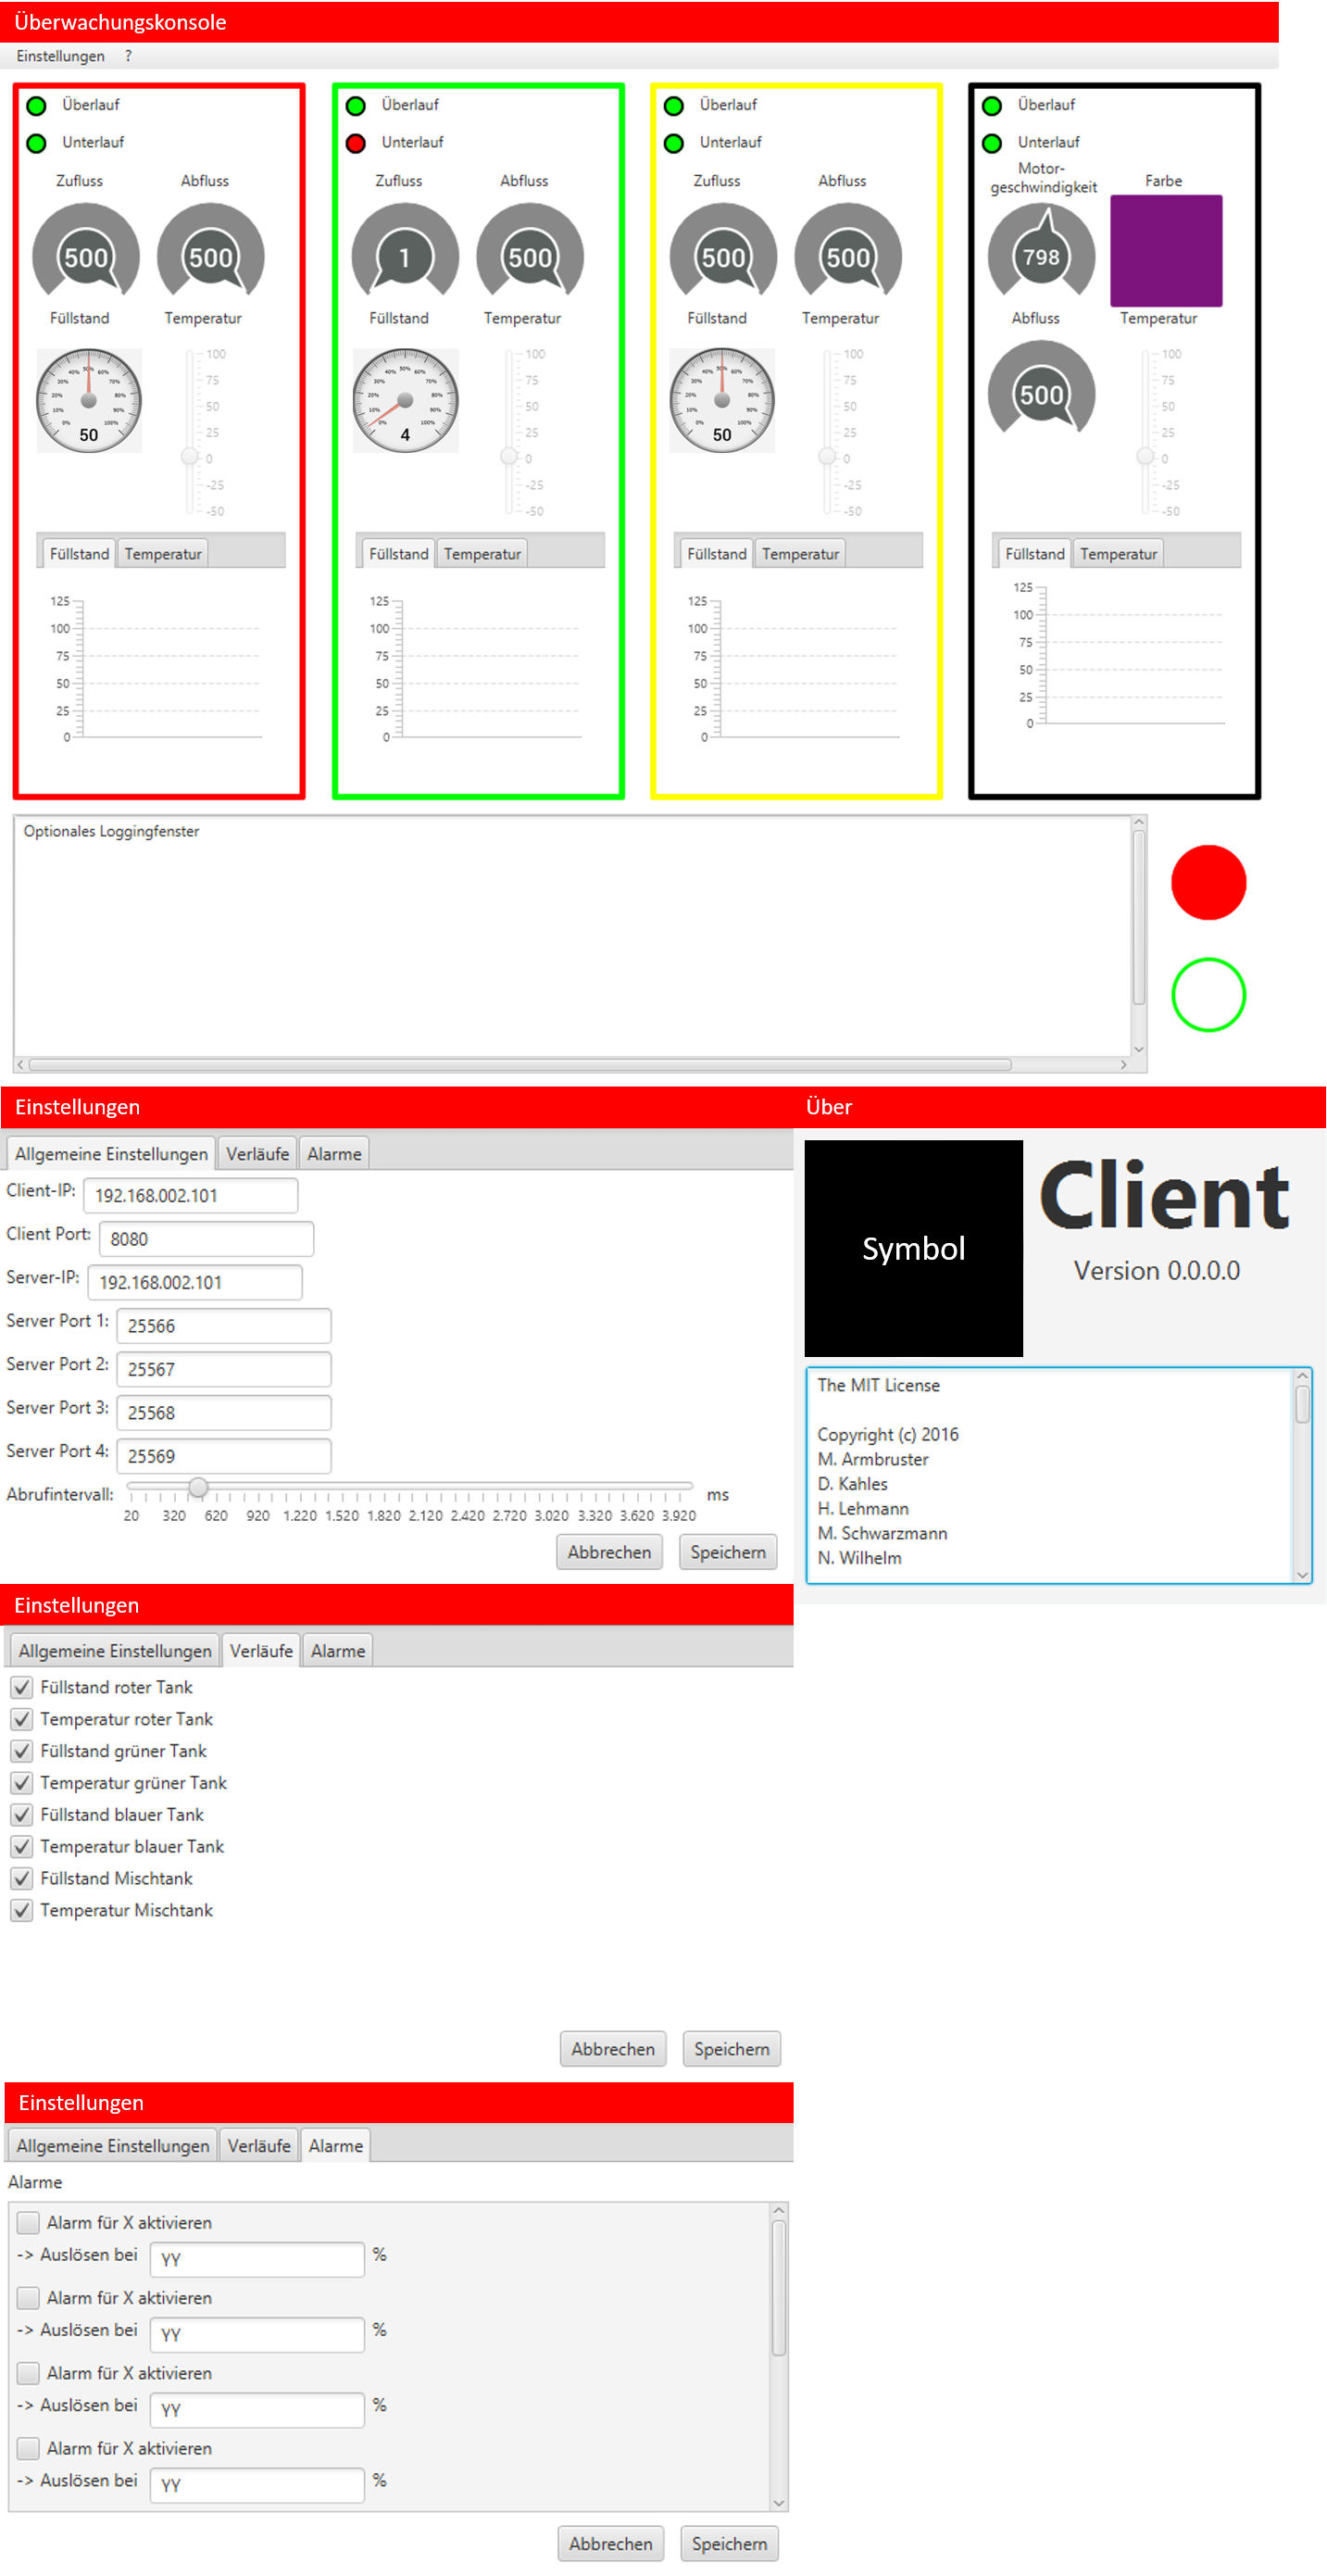
\includegraphics[scale=0.40]{media/ui-client.png}

\section{Anhang}
\subsection{3D-Darstellung der Fertigungssimulation}
Die 3D-Darstellung der \gls{Fertigungssimulation} wurde verworfen, da diese sonst eher wie ein Spiel wirkt.
In der Anwendung soll somit eine schematische Darstellung zum Einsatz kommen.
\begin{center}
  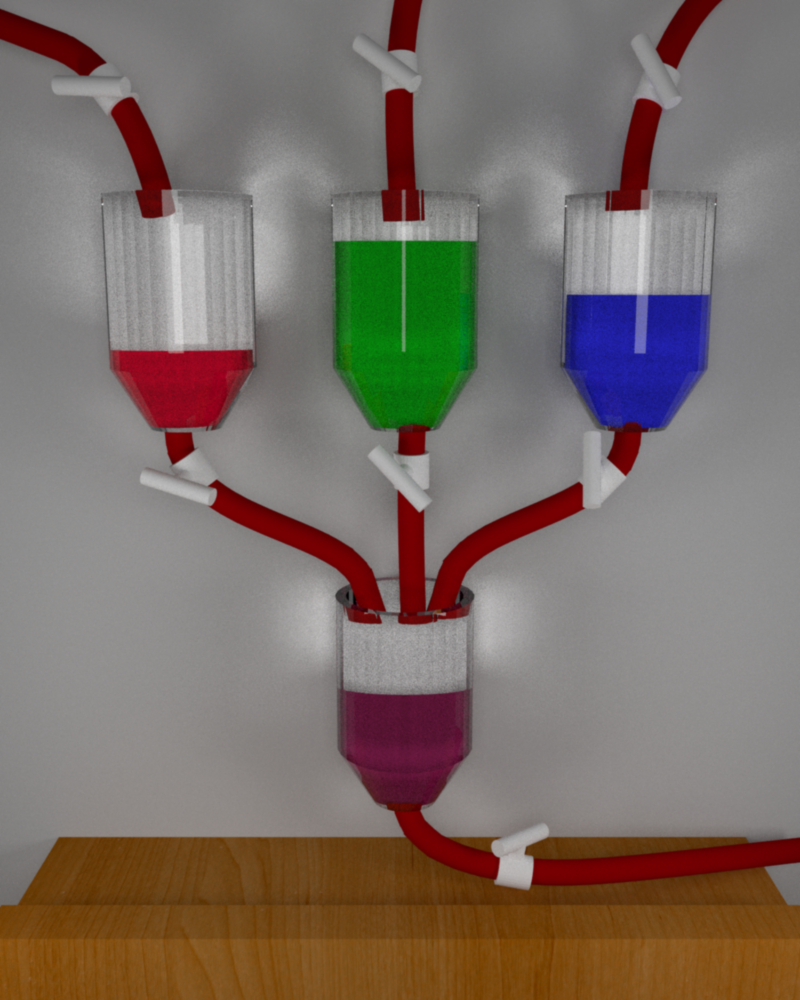
\includegraphics[scale=0.3]{./media/ui-sketch-server-3d.png}
\end{center}

\pagebreak
\printglossaries

\end{document}
